\chapter{A first look}\label{cha:first-look}

Testing the quantum nature of gravity is no easy task and many proposals seek to detect gravitationally induced entanglement between two masses \cite{Krisnanda_2020,Chevalier_2020,Pedernales_2019,Bose_2017} as a form of proof. 
For all these proposals, gravity is assumed to be mediated by a gravitational field.
During a time evolution, this field (like any other external field) can only perform local operations (LO) on the states of the test masses. If gravity is now assumed to behave classically, the propagation between the masses can be described by a classical communication (CC) channel \cite{Lami_2024,Bose_2017}.
These LOCC operations however cannot turn an initially unentangled state into an entangled one \cite{Horodecki_2009, Plenio_2005a}.
It immediately follows, that if one measures the involved masses to be entangled after a mutual gravitational interaction, gravity necessarily has to be quantum in some way.
It is important to note, that the opposite of this statement is not true. Measuring unentangled masses does not directly imply the classicality of the gravitational field.
This can be seen by considering operations that are non-LOCC and also produce unentangled states like for example the swap operation $\ket{\psi}_A\ket{\phi}_B \rightarrow \ket{\phi}_A\ket{\psi}_B$. This operations obviously can't induce entanglement to initially unentangled states, but requires the perfect exchange of quantum information between the states - which is not possible using classical communication alone.
In other words: If one prepares masses initially in a pure product state and measures \textit{any} state which cannot be obtained by LOCC-operations after some final time evolution, it is impossible for gravity to behave classical. One can even go so far and define the term \emph{quantum gravity} as any interaction mediated by gravity that cannot be described by LOCC operations alone \cite{Lami_2024}.

A plausible and logical idea for an experiment to test for gravitational induced entanglement is described in this chapter - which is, as a reminder, enough to prove a quantum nature of gravity.
It requires the generation of coherent delocalized quantum superpositions of massive objects either as so-called Schrödinger-cat states or squeezed gaussian states \cite{Bose_2017, Pedernales_2023}. Theses masses are brought close enough together for gravity to have a measurable effect. The distances between different parts of the spatial superpositions must have different distances to the delocalized second mass. As a result - and of course \textit{if gravity behaves quantum} - the states should get entangled.
To see this, consider the ideal simplification of a real experimental setup where two bodies with mass $m$ are trapped in an harmonic potential wall (like for example in an optical trap) with frequency $\omega$ separated by a distance $d$. The local Hamiltonian of the system is given by
\begin{equation}
  \op{H}_0 = \sum_{i = 1,2} \frac{\op{p}_i^2}{2m} + \frac{1}{2}m\omega^2\op{x}^2_i
\end{equation}
where $\op{x}$ and $\op{p}$ are the position and momentum operators satisfying the canonical commutation relation $[\op{x}_i, \op{p}_j] = i\hbar \delta_{ij}$.
For now, all non-gravitational interactions between the masses have been ignored. 
In the low energy regime, where the energy transfer during a process is far below the Planck scale $m_p c^2 \sim 10^{19}\si{GeV}$, gravity can be traded as an effective field theory with tools available similar to those for the electromagnetic field and QED \cite{Carney_2018}. 
In the non-relativistic limit $v \ll c$, the gravitational interaction can be described by a Newtonian $1/r$ potential acting on the center-of-mass positions, with all classical quantities are replaced by quantum operators \cite{Carney_2018,Pedernales_2023,Christodoulou_2022}. 
Spatial superpositions lead to superpositions of the metric and consequently (in the non-relativistic limit) to a superposed Newtonian potential.
The interaction Hamiltonian $\op{H}_G$ should therefore be describable by
\begin{equation}\label{eq:2:gravity-hamiltonian}
  \op{H}_G = - \frac{Gm^2}{\abs{d - \op{x}_1 + \op{x}_2}} ,
\end{equation}
where $G=6.6743 \times 10^{-11} \si{m^3 kg^{-1} s^{-2}}$ is the gravitational constant. The separation of the masses $d$ is chosen much larger than the extension of the delocalization (in this setup comparable to the position variance of the harmonic oscillator). This condition is realistic given that the biggest spatial delocalization is in the order of !!!SOURCES!!!.
Expanding the Hamiltonian $\op{H}_G$ for small $\op{x}_i$, only the second order term proportional to $(\op{x}_1 - \op{x}_2)^2$ can induce entanglement \cite{Krisnanda_2020}. The zeroth order term is just a overall energy offset, the first order term $\propto (\op{x}_1 - \op{x}_2)$ as well as the terms $\op{x}^2_i$ result only in a local interaction for each mass separately. The coupling term $ - (\op{x}_1\op{x}_2 + \op{x}_2\op{x}_1) = -2\op{x}_1\op{x}_2$ however is very interesting as it couples both oscillators and can thus mediate entanglement.
Introducing the ladder operators, the Hamiltonian $\op{H}=\op{H}_0 + \op{H}_G$ can be expressed as \cite{Carney_2018}:
\begin{equation}\label{eq:2:general-hamiltonian}
  \op{H} = \sum_{i=1,2} \hbar \omega \op{a}_i^\dagger \op{a}_i - \frac{Gm^2}{d^3} \left(\sqrt{\frac{\hbar}{2m\omega}}\right)^2 \left( \op{a}_1\op{a}_2 + \op{a}_1\op{a}^\dagger_2 + \op{a}^\dagger_1\op{a}_2 + \op{a}^\dagger_1\op{a}^\dagger_2 \right)
\end{equation}
Applying the \textit{rotating-wave approximation}\footnote{This approximation is known from quantum optics, where all fast oscillating terms in the Hamiltonian can be dropped \cite{Carney_2018,Lami_2024}. In the interaction picture, the ladder operators evolve as $\op{a}(t) = \op{a}e^{-i\omega t}$. The terms like $\op{a}_1(t)\op{a}_2(t)$ oscillate with frequency $2\omega$ whereas $\op{a}_1^\dagger(t) \op{a}_2(t)$ does not oscillate at all. Due to the small coupling, this approximation works very well here.}, the terms $\op{a}_1\op{a}_2 + \op{a}^\dagger_1\op{a}^\dagger_2$ can be dropped. Defining the coupling strength $g$ of the interaction as $g = Gm/\omega d^3$, eq \eqref{eq:2:general-hamiltonian} can be rewritten as
\begin{equation}
  \op{H} = \sum_{i=1,2} \hbar \omega \op{a}_i^\dagger \op{a}_i - \hbar g \left( \op{a}_1\op{a}^\dagger_2 + \op{a}^\dagger_1\op{a}_2 \right) .
\end{equation}
Now, for simplicity and as a simple example, the evolution of the initial Fock state $\ket{\psi(0)} = \ket{10}$ is considered. The gravitational interaction $H_G$ can be treated as a time dependent perturbation and the state evolution is given as (for calculation see appendix \ref{apx:general-state-perturbation-theory}) \cite{Carney_2018}
\begin{equation} \label{eq:2:general-evolved-state}
  \ket{\psi(t = 0)} = \ket{10} \xrightarrow{\text{time }t} \ket{\psi(t)} =  \mathcal{N} \left(\ket{10} - i g t \ket{01} + \mathcal{O}(g^2) \right)
\end{equation}
where $\mathcal{N}$ is an appropriate normalization constant. The evolved state \eqref{eq:2:general-evolved-state} is entangled and cannot be reduced into a product of two oscillator Fock states. The entanglement is very small since it is proportional to the gravitational coupling constant $gt$ \footnote{The amount of entanglement can for example be measured with the later introduced \textit{logarithmic negativity} $E_N$. For this state, this quantity is given as $E_N(\ketbra{\psi(t)}) \simeq 2tg/\log 2 + \mathcal{O}(g^2) \geq 0$.} but can still be measured by ???? !!!SOURCES!!!.
Another interesting result, which underlines the false inference of a classical gravity from observed non-entanglement discussed above can be seen by considering the time evolution of a coherent product state $\ket{\alpha} \otimes \ket{\beta}$ where $\op{a}\ket{\alpha} = \alpha\ket{\alpha}$. The time evolution is derived in appendix \ref{apx:general-coherent-state-evolution} and results in
\begin{equation}
  e^{-i\op{H}t/\hbar} \left( \ket{\alpha} \otimes \ket{\beta} \right) = \ket{ e^{-i\omega t} \left( \alpha \cos gt - \beta \sin gt \right) }\otimes\ket{ e^{-i\omega t} \left( - \alpha \sin gt + \beta \cos gt \right) } .
\end{equation}
This state is clearly a product state and thus not entangled. But for a time $t_0 = \pi/2g$ the state is effectively the swapped initial state $\ket{\beta} \otimes \ket{\alpha}$ up to a local phase. This swap operation is however, as established earlier, not possible under a LOCC protocol. Thus, even if the resulting state after time evolution under a gravitational interaction is unentangled, we can role out the classicality of gravity \cite{Carney_2018,Lami_2024}. 
Gravity must therefore be capable of transmitting quantum information and must be described by a quantum channel.

Experimentally, one requires the ability to generate spatial superpositions of two massive objects with large enough coherence times. Usually the weak gravitational interaction requires coherence times in the order of $100\si{ms} - 10\si{s}$ for any meaningful and measurable entanglement to built up. The masses should additionally be massive enough for their gravitational effects to be measurable.
These requirements impose huge experimental and engineering challenges. To contextualize: The most massive object ever put into a spatial superposition is in the order of $4 \times 10^{-23}\si{kg}$, whereas the smallest object whose gravitational field has been measured was just below $100 \si{mg}$ \cite{Westphal_2021} - a difference of $19$ orders of magnitude.
One way to experimentally create such spatial superpositions is giving the masses a spin-1/2 degree of freedom. For example, a nitrogen-vacancy diamonds can be used \cite{Bose_2017}, where the NV site provides the required spin of 1/2. An applied magnetic gradient $\partial_x B$ functions like a \q{beam splitter} and creates a delocalized state.
The extend of this superposition can be calculated and separations in the order of $100 \si{\mu m}$ are theoretically achievable \cite{Bose_2017}.
Levitated, trapped particles isolated and shielded in a vacuum can increase environmental isolation by avoiding contact with surrounding noise. The additional forces due to the trapping potential or the gravitational acceleration can be studied in advance. 
In this thesis, I assume that all required states and superpositions can be prepared experimentally.

The general and idealized problem considered is illustrated in \cref{fig:2:simple-problem}.
\begin{figure}[!htbp]
  \centering
  \def\svgwidth{\textwidth}
  \input{./../figures/simple-problem.pdf_tex}
  \caption{Schematic figure of the proposed experiment with two masses prepared in a spatial superposition state. The gravitational interaction $\op{H}$ induces different phases to each of the superpositions due to the different distances between all masses. This results in measurable entanglement after some time evolution.}
  \label{fig:2:simple-problem}
\end{figure}
Two massive bodies with masses $M_A$ and $M_B$ are initially separated by a center-to-center distance $2L$. The masses are prepared in a coherent delocalized quantum superposition Schrödinger-cat-like state in, for now, a parallel orientation as depicted in \cref{fig:2:simple-problem}.
The extension of the superposition is denoted by $\Delta x$ and is the same for both masses.
It is important to choose the positions of the masses such that the distances between each part of the delocalized mass $A$ and $B$ are not always identical. 
Otherwise, all built up phases are the same and no entanglement is observable.
With the notation introduced in \cref{fig:2:simple-problem}, the initial state at $t=0$ is given by
\begin{equation}\label{eq:2:initial-state}
  \ket{\psi(t=0)} = \frac{1}{2}\left( \ket{\psi_A^1} + \ket{\psi_A^2} \right) \otimes \left( \ket{\psi_B^1} + \ket{\psi_B^2} \right) .
\end{equation}
The state evolves under a Hamiltonian $\op{H}$ and after some time the position of each mass is measured and checked for entanglement.
For now I assume that all interactions except gravity can be neglected. In reality, electromagnetic forces and Casimir-Polder interactions \cite{Casimir_1948, Casimir_1948a} need to be considered.

As established earlier in this chapter, with some assumptions made, gravitational interaction can generate entanglement. In the time scales of the experiment, the acceleration of the masses due to the mutual gravitational interaction can be neglected \footnote{Take for example a silica sphere ($\rho = 2648 \si{kg/m^3}$) with $R=10^{-5}\si{m}$ separated by $L=2R$. The mutual gravitational acceleration for each sphere is around $a=GM/(2L)^2 = 5 \times 10^{-13}\si{m/s^2}$ which results for $t\sim 1 \si{s}$ in a distance traveled of $\sim 10^{-13}\si{m}$.}. The Hamiltonian therefore only needs to include the gravitational potential 
\begin{equation} \label{eq:2:potential}
  \op{V} = -\frac{GM_AM_B}{\abs{\op{D}}}
\end{equation}
where $\op{D}$ is the distance operator between the masses. It depends on the individual positions $\op{x}_A$ and $\op{x}_B$.
During time evolution, the different parts of the superpositions built up different local phases. I am interested in calculating, how much entanglement one can expect from this kind of interactions.


\section{Time evolution under a gravitational potential}

\begin{proposition} \label{proposition:time-evolution}
  The time evolution under a static and constant Hamiltonian $\op{H} = \op{V}(\op{x}_i) = \mathrm{const.}$ is given by the eigenenergies of the system $\op{V}\ket{n} = V_n\ket{n}$ proportional to $e^{-iV_nt/\hbar}$.
\end{proposition}
\begin{proof}
  This is a trivial statement. The time evolution is governed by the Schrödinger equation
  \begin{equation}
    i\hbar \pdv{t}\ket{\psi(t)} = \op{H} \ket{\psi(t)} .
  \end{equation}
  The formal solution of this first order PDE is given by
  \begin{equation}
    \ket{\psi(t)} = e^{-i\op{V}t/\hbar} \ket{\psi(t=0)} .
  \end{equation}
  The constant (hermitian) potential operator can be expressed in the energy-eigenbasis $\left\{\ket{n}\right\}$ as $\op{V}\ket{n} = V_n\ket{n}$. The initial state can be expressed as a superposition in the same eigenstates like $\ket{\psi} = \sum_n c_n \ket{\psi_n}$. Putting both together and using the taylor expansion of the exponential function, one arrives at the simple form
  \begin{align}
    \ket{\psi(t)} &= \sum_n e^{-i\op{V}t/\hbar} \ket{n} \braket{n}{\psi} = \sum_{n,k} \frac{(-i\op{V}t/\hbar)^k}{k!} \ket{n} c_n \ket{\psi_n} \\
    &= \sum_{n,k} \frac{(-iV_n t/\hbar)^k}{k!} c_n \ket{\psi_n} 
    = \sum_n e^{-iV_nt/\hbar} c_n \ket{\psi_n}
  \end{align}
  where in the second to last step $\op{V}^k\ket{n} = \op{V}^{k-1}\op{V}\ket{n} = \op{V}^{k-1}\ket{n} V_n = \dots = V_n^k\ket{n}$ was used.
\end{proof}

Using the preceding proposition, the initial state eq. \eqref{eq:2:initial-state} can be evolved in time.
The potential operator eq. \eqref{eq:2:potential} acts on every state in the $\left\{ \ket{\psi_A^1}, \ket{\psi_A^2} \right\}\otimes \left\{ \ket{\psi_B^1}, \ket{\psi_B^2} \right\}$ basis differently. This is because of the different distances between the states $\ket{\psi_A^i}$ and $\ket{\psi_B^j}$ for different $i,j \in \{1, 2\}$. This results in phases $\phi_{ij}$ to be built up during time evolution according to \cref{proposition:time-evolution}.
The state $\ket{\psi(t)}$ after some time evolution is therefore given as
\begin{equation}\label{eq:2:evolved-state}
  \ket{\psi(t)} = \frac{1}{2}\bigl(
    e^{i\phi_{11}} \ket{\psi_A^1}\ket{\psi_B^1} 
    + e^{i\phi_{12}} \ket{\psi_A^1}\ket{\psi_B^2}
    + e^{i\phi_{21}} \ket{\psi_A^2}\ket{\psi_B^1} 
    + e^{i\phi_{22}} \ket{\psi_A^2}\ket{\psi_B^2} \bigr) ,
\end{equation}
where the $\otimes$ symbol was omitted. The phases are
\begin{align}
  \phi \equiv \phi_{11} = \phi_{22} = \frac{G M_A M_B}{2\hbar L}t 
  \qquad \text{and} \qquad 
  \phi_{12} = \phi_{21} = \frac{G M_A M_B}{\hbar \sqrt{4L^2 + (\Delta x)^2}}t .
\end{align}
Assuming again that the superposition size $\Delta x$ is much smaller than the distance $L$ between the masses - like before in eq. \eqref{eq:2:gravity-hamiltonian} - the phases $\phi_{12}=\phi_{21}$ can be expanded and a global phase $\phi$ can be factored:
\begin{equation}\label{eq:2:definition-delta-phi}
  \phi_{12} = \phi_{21} \approx \frac{GM_AM_B}{\hbar} \left[ \frac{1}{2L} - \frac{(\Delta x)^2}{16 L^3} \right] t \equiv \phi - \Delta\phi .
\end{equation}
The state eq. \eqref{eq:2:evolved-state} can now be expressed in the form
\begin{equation}
  \ket{\psi(t)} = e^{i\phi}\frac{1}{\sqrt{2}}\left[ 
    \ket{\psi_A^1} \otimes \frac{\ket{\psi_B^1} + e^{-i\Delta\phi} \ket{\psi_B^2}}{\sqrt{2}}
    + \ket{\psi_A^2} \otimes \frac{e^{-i\Delta\phi} \ket{\psi_B^1} + \ket{\psi_B^2}}{\sqrt{2}} \right] ,
\end{equation}
where the entanglement dynamics can be directly seen. This state is entangled, if it is not representable as a product state $\ket{\psi} \neq \ket{\psi_A}\otimes\ket{\psi_B}$. That is the case, if the states containing $\ket{\psi_B^i}$ are not both equal to each other (i.e. differ only by a phase) and thus cannot be factored. 
The system is therefore entangled, if and only if $\Delta\phi \neq k\pi$ with integer $k \in \mathbb{Z}$.


% \section{Fidelity of quantum states}
% In general, to compare the distance between two quantum states $\rho$ and $\sigma$ (\q{how similar they are}) the \emph{fidelity} $F(\rho, \sigma)$ is used. It is defined as \cite[p. 409-412]{Nielsen_2010} 
% \begin{equation}
%   F(\rho, \sigma) = \tr \sqrt{\sqrt{\rho} \sigma \sqrt{\rho}}
% \end{equation} 
% and can be used as a distance measurement between quantum states. It is monotonic, concave and bounded between 0 and 1. If both states are equal $\rho = \sigma$, it is clear that $F(\rho, \sigma) = 1$, by using $\sqrt{\rho}\rho\sqrt{\rho} = \rho^2$. If both states commute, i.e. they are diagonalizable in the same orthogonal basis $\{ \ket{i} \}$, 
% \begin{equation*}
%   \rho = \sum_i r_i \ketbra{i}; \quad \sigma = \sum_i s_i \ketbra{i},
% \end{equation*}
% the fidelity is given by \cite[p. 409]{Nielsen_2010}
% \begin{equation*}
%   F(\rho, \sigma) = \tr \sqrt{\sum_i r_i s_i \ketbra{i}} = \sum_i \sqrt{r_i s_i}.
% \end{equation*}
% This can be seen immediately by the use of the spectral theorem $\tr \sqrt{\rho} = \tr{U \sqrt{\mathrm{diag}(r_i)} U^\dagger} = \tr \diag(\sqrt{r_i})$.
% Another special case is given for the fidelity of a pure state $\rho=\ketbra{\psi}$ and an arbitrary state $\sigma$ \cite[p. 409]{Nielsen_2010}:
% \begin{equation*}
%   F(\ket{\psi}, \sigma) = \tr \sqrt{\bra{\psi}\sigma\ket{\psi} \ketbra{\psi}} = \sqrt{\bra{\psi}\sigma\ket{\psi}}.
% \end{equation*}
% If the state $\sigma = \ketbra{\phi}$ is also pure, the fidelity reduces to
% \begin{equation*}
%   F(\ket{\psi}, \ket{\phi}) = \abs{\braket{\psi}{\phi}} \le 1,
% \end{equation*}
% with equality being attained if the states are the same and only differ by a phase. 
In order to assess in a more quantitative way how entangled the state $\ket{\psi}$ is, a more sophisticated entanglement measure is needed. In the next chapter, the \emph{logarithmic negativity} is motivated and introduced. In the rest of this thesis, I will repeatedly opt for this measure.


\section{Entanglement measures}
Checking whether an arbitrary state $\rho$ is entangled or not is no easy task. In fact, this problem is known to be NP-hard \cite{Gurvits_2003}.
A state $\rho_{AB} \in \mathcal{H}_A\otimes\mathcal{H}_B$ is called entangled, if it is \emph{non-separable}, that is, it cannot be expressed as a tensor product of two subsystems $\rho_A \in \mathcal{H}_A$ and $\rho_B \in \mathcal{H}_B$.
Only for specific cases - like the case of two qubits or qubit-qutrit - a simple sufficient criterion for determining the separability of a general mixed state is known:
The positive partial transpose (PPT) criterion states, that if the partial transpose of the density matrix is positive ($\rho^{\Gamma_A} > 0$ \footnote{A matrix is defined as positive (\q{positive definite}), if all eigenvalues are positive.}), the state $\rho$ is separable \cite{Horodecki_2009,Plenio_2005a}. In other words, if $\rho^{\Gamma_A}$ has negative eigenvalues, $\rho$ is guaranteed to describe an entangled state.
The inverse is true, if and only if the dimension of $\rho_A\otimes\rho_B$ is $2\times2$ or $3\times2$ \cite{Horodecki_2009} - otherwise, only having non-negative eigenvalues doesn't necessarily result in an unentangled system (such states are called \q{bound states}).
The partial transpose with respect to a subsystem $i$ can be understood in the same way as the partial trace, where the operation (in this case the transform) is performed only on indices corresponding the subsystem $\rho_i$.
To see the necessity of the PPT criterion, consider a separable mixed state $\rho$, which can be generally expressed as 
\begin{equation}\label{eq:2:separable-state}
  \rho = \sum p_i \rho_{A}^i\otimes\rho_{B}^i .
\end{equation}
The partial transpose is in this case trivial:
\begin{equation}
  \rho^{\Gamma_A} = \sum p_i (\rho_{A}^i)^T \otimes \rho_{B}^i .
\end{equation}
Since the transpose preserves eigenvalues, the transposed subsystem $A$ is still positive $(\rho_{A}^i)^T > 0$ and describes again a valid quantum state. It follows, that $\rho^{\Gamma_A}$ is positive as well.
If somehow $\rho^{\Gamma_A}$ has any negative eigenvalues, this can only mean that the initial state $\rho$ is not separable and cannot be expressed in the form of eq. \eqref{eq:2:separable-state} and the necessity of the criterion is shown.

For quantifying entanglement in a more precise way, a mathematical quantity called \emph{entanglement measure} can be used. A good measure should be able to capture the essential features of entanglement. One can axiomatically state what properties such a measure $E(\rho)$ should have \cite{Plenio_2005a,Horodecki_2009}:
\begin{description}
  \item[Normalization] An entanglement measure should be a mapping from densities to real positive values between 0 and 1:
  \begin{equation}
    \rho \rightarrow E(\rho) \in \mathbb{R}^+
  \end{equation}
  where usually the maximally entangled state has $E=1$.
  \item[Monotonicity under LOCC] $E$ should not increase under local operations and classical communications. This is the most important postulate for an entanglement measure and often cited as the \textit{only} required postulate.
  \item[Vanishing on separable states] $E(\rho)=0$ if $\rho$ is separable
  \item[] Often one finds additional properties useful like \textit{convexity} $E(\sum p_i \rho_i) \leq \sum p_i E(\rho_i)$ or (full) \textit{additivity} $E(\rho \otimes \sigma) = E(\rho) + E(\sigma)$.
\end{description}
A function that satisfies the most important of these conditions is often called an \textit{entanglement monotone}.

The \emph{negativity} $\mathcal{N}$ is such an entanglement monotone \cite{Vidal_2001,Plenio_2005a} that used the PPT criterion to determine if a state is entangled or not. It is defined as 
\begin{equation}\label{eq:2:negativity}
  \mathcal{N} = \frac{\norm{\rho^{\Gamma_A}}_1 - 1}{2}
\end{equation}
where $\norm{A}_1 = \tr\abs{A} = \tr \sqrt{A^\dagger A}$ is the trace norm. The negativity however is not additive and a more suitable and widely used entanglement measure is the \emph{logarithmic negativity} \cite{Plenio_2005,Horodecki_2009,Plenio_2005a}
\begin{equation}\label{eq:2:logarithmic-negativity}
  E_N(\rho) = \log_2\norm{\rho^{\Gamma_A}}_1 .
\end{equation}
The monotonicity of the logarithm implies, that $E_N$ is an entanglement monotone as well.
Furthermore, for the calculations it does not matter which subsystem is transposed.

\begin{proposition}
  a) The partial transpose w.r.t. subsystem $A$ is equal to the transposed partial transpose w.r.t. subsystem $B$: $\rho^{\Gamma_A} = (\rho^{\Gamma_B})^T$. 
  b) The trace norms of partially transposed density operators w.r.t. any subsystem are equal: $\norm{\rho^{\Gamma_A}}_1 = \norm{\rho^{\Gamma_B}}_1$.
\end{proposition}
\begin{proof}
  a) A general density matrix $\rho$ can be expressed as
  \begin{equation*}
    \rho = \sum_{i,j,k,l} \rho_{ij,kl} \ketbra{i}{j}_A\otimes\ketbra{k}{l}_B
  \end{equation*}
  The partial transpose with respect to subsystem $B$ is then defined as 
  \begin{equation*}
    \rho^{\Gamma_B} \equiv \sum_{i,j,k,l} \rho_{ij,kl} \ketbra{i}{j}_A\otimes\left(\ketbra{k}{l}_B\right)^T = \sum_{i,j,k,l} c_{ij,kl} \ketbra{i}{j}_A\otimes\ketbra{l}{k}_B
  \end{equation*}
  The complete transpose of this is
  \begin{equation*}
    (\rho^{\Gamma_B})^T = \sum_{i,j,k,l} \rho_{ij,kl} \left(\ketbra{i}{j}_A\right)^T\otimes\left(\ketbra{l}{k}_B\right)^T = \sum_{i,j,k,l} c_{ij,kl} \ketbra{j}{i}_A\otimes\ketbra{k}{l}_B \equiv \rho^{\Gamma_A}
  \end{equation*}
  b) Clear by a) and by using \cref{lemma:trace-norm-hermitian} and the fact that the eigenvalues of a square matrix $A$ and $A^T$ are equal.
\end{proof}

The logarithmic negativity is very easy to calculate compared to other entanglement measures. It is enough to compute the square root of the eigenvalues of $(\rho^{\Gamma})^\dagger \rho^{\Gamma}$ or the absolute sum of the eigenvalues of $\rho^{\Gamma}$.
For practical and numeric calculations it is often more easy and stable to take a single eigenvalue than the need to compute the sum of multiple. 
For all numerical calculations in this thesis, I therefore opt for an alternative way to compute the logarithmic negativity.

\begin{lemma}\label{lemma:trace-norm-hermitian}
  The trace norm $\norm{A}_1 \equiv \tr \sqrt{A^\dagger A}$ of a hermitian matrix $A$ is equal to the sum of the absolute eigenvalues of $A$.
\end{lemma}
\begin{proof}
  This can be immediately seen by the spectral theorem:
  \begin{equation*}
    \tr \sqrt{A^\dagger A} = \tr \sqrt{A^2} = \tr{U\sqrt{\diag(\lambda_1, \dots)^2}U^\dagger} = \sum_i \sqrt{\lambda_i^2} = \sum_i \abs{\lambda_i}.
  \end{equation*}
\end{proof}

\begin{proposition}\label{proposition:negativity}
  The negativity eq. \eqref{eq:2:negativity} is given as the absolute sum of all negative eigenvalues of $\rho^{\Gamma}$: 
\begin{equation}
    \mathscr{N}(\rho) \equiv \frac{\norm{\rho^{\Gamma}}_1 - 1}{2} = \abs{\sum_{\lambda_i < 0} \lambda_i}.
\end{equation}
\end{proposition}
\begin{proof}
  The proof is in parts given by Vidal and Werner \cite{Vidal_2001}. It is known that the density matrix is hermitian: $\rho = \rho^\dagger$. Using \cref{lemma:trace-norm-hermitian}, the trace norm of the density matrix is is given as $\norm{\rho}_1=\sum \lambda_i = \tr \rho = 1$. The partial transpose $\rho^{\Gamma}$ obviously also satisfies $\tr \rho^{\Gamma} = 1$ but might have negative eigenvalues. Since $\rho^{\Gamma}$ is still hermitian, the trace norm is given by
  \begin{equation*}
    \norm{\rho^{\Gamma}}_1 = \sum_i\abs{\lambda_i} = \sum_{\lambda_i \ge 0} \lambda_i + \sum_{\lambda_i < 0} \abs{\lambda_i} = \sum_i \lambda_i + 2\sum_{\lambda_i < 0} \abs{\lambda_i} = 1 + 2\sum_{\lambda_i < 0} \abs{\lambda_i} ,
  \end{equation*}
  where in the last step $\sum \lambda_i = \tr \rho^{\Gamma} = 1$ was used. The negativity can be defined as $\mathscr{N}(\rho) = \abs{\sum_{\lambda_i < 0} \lambda_i}$ and the statement is shown.
\end{proof}
\begin{remark}
  The PPT criterion states, that if $\rho^{\Gamma}$ has negative eigenvalues, the state $\rho$ is entangled. The negativity uses this criterion for a quantification of entanglement. This proposition makes sense of the name \textit{negativ}ity.
\end{remark}

Calculating the logarithmic negativity of the evolved state eq. \eqref{eq:2:evolved-state}, it is possible to quantify how the entanglement behaves in time. A straight forward computation following the calculation methods established above yields (for detailed calculations see appendix \ref{apx:E_N-exemplary})
\begin{equation}\label{eq:2:entanglement-dynamics-parallel}
  E_N(\ketbra{\psi(t)}) = \log_2\left(1 + \abs{\sin \Delta\phi}\right) .
\end{equation}
It is interesting to see, that the maximum entanglement $E_N = 1$ is reached for $\Delta\phi = 2\pi k \pm \pi/2, \, k\in\mathbb{Z}$ and no entanglement ($E_N=0$) is measurable for $\Delta\phi = k\pi$. This result aligns with the previous observations by demanding that the evolved state eq. \eqref{eq:2:evolved-state} is separable.
The complete entanglement dynamics are shown in \cref{fig:2:entanglement-dynamics}.
\begin{figure}[!htbp]
  \centering
  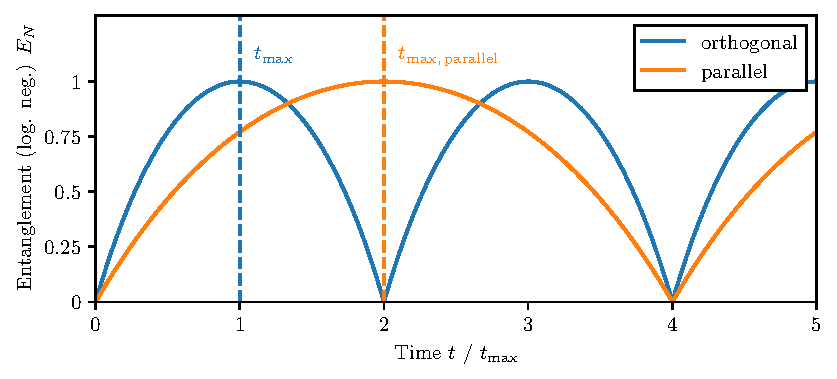
\includegraphics[width=\textwidth]{./../figures/ideal-entanglement/EN-time.pdf}
  \caption{Entanglement dynamics quantified by the logarithmic negativity for two different orientations of the spatial superpositions. The parallel orientation was considered in this chapter (see eq. \eqref{eq:2:entanglement-dynamics-parallel}), the \q{orhtogonal} one in Ref. \cite{Pedernales_2023}. The time of maximum entanglement $t_\mathrm{max}$ for the orthogonal configuration is reached after $t_\mathrm{max} = 4\pi\hbar L^3 / (G M_A M_B \Delta x^2) \simeq 129\si{ms}$.}
  \label{fig:2:entanglement-dynamics}
\end{figure}
The time $t_\mathrm{max,\,parallel}$ at which the entanglement is maximal (for the first time) can be calculated by using the definition of $\Delta\phi$ from eq. \eqref{eq:2:definition-delta-phi} as
\begin{equation}
  t_\mathrm{max,\,parallel} = \frac{8 \pi L^3\hbar}{G M_A M_B (\Delta x)^2} .
\end{equation}
In \cref{fig:2:entanglement-dynamics} the entanglement dynamics for a different orientation considered in Ref. \cite{Pedernales_2023} is also shown. 
There, the superpositions are aligned in the same line as the direct connection between the masses (\q{orthogonal} to the parallel configuration before), maximizing the differences in distances between them and thus creating entanglement faster. This expected behavior can be well seen in \cref{fig:2:entanglement-dynamics}: The time $t_\mathrm{max}$ until the maximum entanglement is reached, is precisely by a factor of $2$ faster than in the here considered parallel configuration \cite{Pedernales_2023}. 
For a practical experiment, this suggests that using the orthogonal orientation could be beneficial and would require shorter coherence times for the superpositions.
To give an estimate, consider two identical silica spheres with a density of $\rho=2648\si{kg/m^3}$ with a radius of $R=10^{-5}\si{m}$, a separation of $2L = 4R$ and a superposition size $\Delta x = 100\si{nm}$ (which is realistic considering theoretical sizes of up to micrometers \cite{Bose_2017}), the maximum entanglement is reached after about $t_\mathrm{max} \approx 129\si{ms}$ which is a quite long coherence time and challenging experimentally.


\section{Issues with the experimental procedure}

Additional effects:
- Casimir forces entangle as well
- Coulomb forces

-> solution: conducting faraday shield, UV discharge \cite{Kamp_2020}

How to measure? Many measurements are necessary -> Entanglement witness? Measure density directly -> Small variations for each measurement in angle of the superposition and in distance to the newly introduced shield